%%
%% CS 203 -- Project 5: Voice Helpdesk ASR -- ASSIGNMENT 2 REPORT
%% Model Development, Deployment and Monitoring
%% Build: pdflatex report_A2 && bibtex report_A2 && pdflatex report_A2 && pdflatex report_A2
%% Figures fig_a2_*.pdf come from code/scripts/make_report_figures.py;
%% tables tab_*.tex are auto-generated from the result files; numbers live in numbers.tex.
%%
\documentclass[sigconf,authordraft]{acmart}
\AtBeginDocument{\providecommand\BibTeX{{Bib\TeX}}}
\setcopyright{acmlicensed}
\copyrightyear{2026}\acmYear{2026}
\acmDOI{XXXXXXX.XXXXXXX}
\acmConference[CS 203 A2 '26]{CS 203 Software Tools and Techniques in AI -- Assignment 2}{2026}{Gandhinagar, India}
\acmISBN{978-1-4503-XXXX-X/2026/11}
%% common.tex -- shared packages / macros for both reports
\usepackage{booktabs}
\usepackage{amsmath}
\usepackage{xcolor}
\usepackage{url}
\usepackage{graphicx}
\usepackage{array}
\usepackage{multirow}
\usepackage{tikz}
\usetikzlibrary{arrows.meta,positioning,shapes.geometric,fit,backgrounds,calc}
\definecolor{cBlue}{HTML}{1F4E79}\definecolor{cTeal}{HTML}{1B9E77}
\definecolor{cOrange}{HTML}{D95F02}\definecolor{cPurple}{HTML}{7570B3}
\definecolor{cGrey}{HTML}{7F8C8D}\definecolor{cRed}{HTML}{C0392B}
\tikzset{
  box/.style={draw=cBlue,fill=cBlue!8,rounded corners=2pt,align=center,font=\scriptsize,inner sep=3pt,minimum height=0.9cm,text width=2.1cm},
  boxT/.style={box,draw=cTeal,fill=cTeal!10},
  boxO/.style={box,draw=cOrange,fill=cOrange!10},
  boxP/.style={box,draw=cPurple,fill=cPurple!10},
  boxR/.style={box,draw=cRed,fill=cRed!8},
  arr/.style={-{Stealth[length=4pt]},thick,color=cGrey},
  lab/.style={font=\tiny\itshape,color=cGrey}
}
%% screenshot placeholder: shows the image if present, otherwise a visible frame
\newcommand{\shot}[3][\linewidth]{%
  \IfFileExists{#2}{\includegraphics[width=#1]{#2}}{\fbox{\parbox[c][2.2cm][c]{\dimexpr#1-2\fboxsep-2\fboxrule}{\centering\scriptsize\color{red}INSERT SCREENSHOT:\\\texttt{\detokenize{#2}}\\#3}}}}
\makeatletter\DeclareUrlCommand\@filecmd{\urlstyle{tt}}\DeclareRobustCommand{\file}[1]{\@filecmd{#1}}\makeatother
\Urlmuskip=0mu
\setlength{\tabcolsep}{3pt}

%% =====================================================================
%% numbers.tex  --  SINGLE PLACE to update numbers after you re-run things.
%% Values below are copied from the updated repository snapshot
%% (supporting_files/evaluation_results.json, TEST_SET_LOG.md, ...).
%% =====================================================================
\newcommand{\TBD}[1]{{\color{red}\textbf{[TBD: #1]}}}

%% ---- Assignment 1: agreement (recomputed from supporting_files/label_studio_exports)
\newcommand{\KapOne}{0.723}      % round 1, guidelines v1, n=120
\newcommand{\KapTwo}{0.845}      % round 2, guidelines v2, n=120
\newcommand{\DisOne}{25}
\newcommand{\DisTwo}{14}
\newcommand{\AgrOne}{79.2\%}
\newcommand{\AgrTwo}{88.3\%}

%% ---- Assignment 1: Full 182-clip double-annotation & expert adjudication (final_annotation/)
\newcommand{\TotalCorpusClips}{182}
\newcommand{\CorpusHours}{1.82}     % 1h 49m 20.31s total acoustic duration
\newcommand{\KapFinal}{0.656}       % Cohen's kappa n=182 full corpus
\newcommand{\KapFinalCI}{[0.571, 0.741]}
\newcommand{\AgrFinal}{74.2\%}      % 135/182 concordant annotations
\newcommand{\DisFinal}{47}          % 47 residual boundary disputes
\newcommand{\PabakFinal}{0.484}
\newcommand{\LangJaccard}{79.5\%}
\newcommand{\GujaratiAgr}{93.0\%}
\newcommand{\HindiAgr}{76.8\%}
\newcommand{\EnglishAgr}{61.1\%}
\newcommand{\AdjudicationTasks}{47} % tasks routed to annotator_expert on port 8083
\newcommand{\ExpertTasks}{55}       % 47 unique disputes + 8 hidden test-retest repeats
\newcommand{\ExpertDisputes}{47}
\newcommand{\ExpertRepeats}{8}
\newcommand{\ExpertRepeatPct}{17.0\%}
\newcommand{\ExpertMinSep}{35}      % minimum task separation distance for test-retest
\newcommand{\ExpertCompletePct}{100.0\%}
\newcommand{\ExpertMeanLead}{153.8\,s}
\newcommand{\ExpertMedianLead}{79.2\,s}
\newcommand{\IntraRaterKappa}{0.652}
\newcommand{\IntraRaterAgr}{75.0\%}
\newcommand{\GoldAdmissions}{35}
\newcommand{\GoldHostelMess}{54}
\newcommand{\GoldITSupport}{35}
\newcommand{\GoldStudentServices}{58}

%% ---- Assignment 1: relabelling-from-audio results
\newcommand{\RelabKapOne}{0.723}
\newcommand{\RelabKapTwo}{0.845}
\newcommand{\RelabWER}{0.002}

%% ---- Assignment 2: gold (original references, SHA-256 frozen)
\newcommand{\GoldWER}{1.272}   \newcommand{\GoldWERci}{[1.156, 1.393]}
\newcommand{\GoldCER}{0.945}   \newcommand{\GoldCERci}{[0.891, 1.006]}
\newcommand{\GoldAcc}{24.0\%}  \newcommand{\GoldAccci}{[10.3, 41.4]}
\newcommand{\GoldFone}{0.225}  \newcommand{\GoldFoneci}{[0.083, 0.389]}
\newcommand{\GoldBaccOne}{31.0\%} \newcommand{\GoldBaccOneci}{[13.8, 48.3]}
%% ---- gold, acoustically corrected (data/gold_corrections.csv)
\newcommand{\CorrWER}{1.298}   \newcommand{\CorrWERci}{[1.088, 1.501]}
\newcommand{\CorrCER}{1.008}   \newcommand{\CorrCERci}{[0.855, 1.150]}
\newcommand{\CorrAcc}{30.8\%}  \newcommand{\CorrAccci}{[13.8, 48.3]}
\newcommand{\CorrFone}{0.261}  \newcommand{\CorrFoneci}{[0.127, 0.393]}
\newcommand{\CorrBaccOne}{41.5\%} \newcommand{\CorrBaccOneci}{[24.1, 58.6]}
%% ---- validation / cohort B / augmented
\newcommand{\ValWER}{1.403}  \newcommand{\ValWERci}{[1.225, 1.601]}
\newcommand{\ValCER}{1.050}  \newcommand{\ValCERci}{[0.968, 1.143]}
\newcommand{\ValAcc}{53.5\%} \newcommand{\ValAccci}{[29.4, 76.5]}
\newcommand{\ValFone}{0.451} \newcommand{\ValFoneci}{[0.226, 0.637]}
\newcommand{\ValBaccOne}{29.7\%} \newcommand{\ValBaccOneci}{[11.8, 52.9]}
\newcommand{\CbWER}{1.104}   \newcommand{\CbWERci}{[1.040, 1.187]}
\newcommand{\CbCER}{0.947}   \newcommand{\CbCERci}{[0.900, 0.994]}
\newcommand{\CbAcc}{25.2\%}  \newcommand{\CbAccci}{[12.5, 40.6]}
\newcommand{\CbFone}{0.219}  \newcommand{\CbFoneci}{[0.089, 0.359]}
\newcommand{\CbBaccOne}{25.2\%} \newcommand{\CbBaccOneci}{[12.5, 40.6]}
\newcommand{\AugWER}{1.684}  \newcommand{\AugWERci}{[1.590, 1.786]}
\newcommand{\AugCER}{1.060}  \newcommand{\AugCERci}{[1.012, 1.113]}
\newcommand{\AugAcc}{63.5\%} \newcommand{\AugAccci}{[51.7, 75.0]}
\newcommand{\AugFone}{0.613} \newcommand{\AugFoneci}{[0.488, 0.738]}
\newcommand{\AugBaccOne}{26.6\%} \newcommand{\AugBaccOneci}{[16.7, 38.3]}
%% ---- latency (supporting_files/loadtest/latency_profile.json, offline_validation_output.json)
\newcommand{\LatP}{2.86}  \newcommand{\LatPn}{7.69} \newcommand{\LatPf}{13.44} \newcommand{\LatMean}{4.39}
\newcommand{\RTF}{0.243}  \newcommand{\Thr}{0.23}   \newcommand{\PeakMB}{783}
%% ---- Docker measurements
\newcommand{\ImgSize}{3.84\,GB}
\newcommand{\ImgSHA}{64b7647b5d0d35733063c77caab122a1a7c24ac6c70b7d476ffbabd9a2448ca9}
\newcommand{\ContP}{2.86\,s / 13.44\,s}
\newcommand{\ContRAM}{783\,MB}

%% ---- Multilingual Model Pipeline & Offline ASR (model/)
\newcommand{\CuratedClips}{182}
\newcommand{\CuratedHours}{1.82}
\newcommand{\CuratedUnique}{182}
\newcommand{\OfflineASRClips}{182}
\newcommand{\OfflineASRMinutes}{109.3}
\newcommand{\OfflineASRComputeMin}{23.8}
\newcommand{\OfflineASRRTF}{0.218}
\newcommand{\OfflineASRWER}{1.617}
\newcommand{\OfflineASRCER}{1.266}
\newcommand{\OfflineASRMatch}{32.1\%}
\newcommand{\OfflineGujaratiWER}{0.553}
\newcommand{\OfflineGujaratiCER}{0.387}
\newcommand{\OfflineGujaratiMatch}{41.0\%}
\newcommand{\OfflineEnglishWER}{1.169}
\newcommand{\OfflineEnglishCER}{0.927}
\newcommand{\OfflineEnglishMatch}{59.6\%}
\newcommand{\OfflineHindiWER}{2.558}
\newcommand{\OfflineHindiCER}{1.942}
\newcommand{\OfflineHindiMatch}{10.2\%}
\newcommand{\OfflineCodeMixedWER}{2.078}
\newcommand{\OfflineCodeMixedCER}{1.833}
\newcommand{\AugGenerated}{461}
\newcommand{\AugGateOneRej}{95}
\newcommand{\AugGateTwoRej}{34}
\newcommand{\AugGateThreeRej}{208}
\newcommand{\AugAccepted}{124}
\newcommand{\AugTotalPool}{306}
\newcommand{\LeakageAuditorStatus}{PASS (Zero Contamination)}
\newcommand{\AblationBaselineAcc}{58.3\%}
\newcommand{\AblationBaselineFOne}{0.582}
\newcommand{\AblationPivotLatinAcc}{60.5\%}
\newcommand{\AblationPivotLatinFOne}{0.604}
\newcommand{\AblationTopThreeAcc}{56.6\%}
\newcommand{\AblationTopThreeFOne}{0.560}
\newcommand{\AblationFullAcc}{54.6\%}
\newcommand{\AblationFullFOne}{0.553}
\newcommand{\UnseenBenchmarkAcc}{46.0\%}
\newcommand{\UnseenBenchmarkFOne}{0.468}
\newcommand{\UnseenEnglishFOne}{0.886}
\newcommand{\UnseenGujaratiFOne}{0.232}
\newcommand{\UnseenHindiFOne}{0.240}
\newcommand{\UnseenCodeMixedFOne}{0.333}

\begin{document}

\title[Project 5 -- Assignment 2: Voice Helpdesk ASR]{%
  Evaluating, Deploying and Monitoring a Code-Mixed Voice Helpdesk Pipeline:
  Whisper Routing, Experiment Tracking, Offline Docker Serving and a Gated Retraining Loop}

\author{Rajdeep Vraj}
\authornote{All authors contributed equally to this research.}
\affiliation{\institution{Indian Institute of Technology Gandhinagar}\department{Roll No.\ 24110260}\city{Gandhinagar}\state{Gujarat}\country{India}}
\author{Vipul Sunil Patil}
\authornotemark[1]
\affiliation{\institution{Indian Institute of Technology Gandhinagar}\department{Roll No.\ 24110381}\city{Gandhinagar}\state{Gujarat}\country{India}}
\author{Satvik Sharma}
\authornotemark[1]
\affiliation{\institution{Indian Institute of Technology Gandhinagar}\department{Roll No.\ 24110300}\city{Gandhinagar}\state{Gujarat}\country{India}}
\renewcommand{\shortauthors}{Vraj, Patil and Sharma}

\begin{abstract}
We implement, track, evaluate and deploy a lightweight voice-helpdesk pipeline: Whisper-base transcription feeding a TF-IDF + MLP intent router with four classes, served offline on CPU through FastAPI and Streamlit, with drift monitoring and a gated active-retraining loop.
Over 15 MLflow-tracked search runs, validation accuracy ranges from 29\% to 53\% (selected on validation only), and all results carry 95\% bootstrap intervals on validation, test/gold, corrected gold, Cohort~B and augmented data.
Our central result is \emph{negative and diagnostic}: the ASR stage is unadapted Whisper-base, WER on the gold set is \GoldWER{} \GoldWERci{} (more than 1, i.e.\ worse than emitting nothing), proposed and baseline ASR are identical on every clip, and intent accuracy (\GoldAcc{} gold, \CbAcc{} Cohort~B) is statistically indistinguishable from 25\% chance. A WER decomposition shows 83\% substitutions and only 14 of 838 reference words recovered, which we trace to template-derived reference transcripts (Assignment~1 audit) and to code-mixed speech that the base model cannot transcribe.
The monitoring replay shows that neither label-free signal separates drifted from in-domain traffic (r $\le0.41$, $n{=}5$ batches), and the one logged alert is produced by a schedule clause, which we disclose rather than count as detection.
The gated retraining pipeline demonstrates promotion, rejection and rollback mechanics, but its promotion rests on one clip of 13 and we treat it as a mechanism demonstration, not an improvement claim.
We specify the fixes that these findings call for and the evidence needed for each claim.
\end{abstract}

\begin{CCSXML}
<ccs2012>
 <concept><concept_id>10010147.10010178.10010179</concept_id><concept_desc>Computing methodologies~Speech recognition</concept_desc><concept_significance>500</concept_significance></concept>
 <concept><concept_id>10011007.10011074.10011099</concept_id><concept_desc>Software and its engineering~Software verification and validation</concept_desc><concept_significance>300</concept_significance></concept>
 <concept><concept_id>10010147.10010257</concept_id><concept_desc>Computing methodologies~Machine learning</concept_desc><concept_significance>300</concept_significance></concept>
</ccs2012>
\end{CCSXML}
\ccsdesc[500]{Computing methodologies~Speech recognition}
\ccsdesc[300]{Software and its engineering~Software verification and validation}
\ccsdesc[300]{Computing methodologies~Machine learning}
\keywords{Whisper; code-mixed ASR; MLOps; MLflow; Docker; drift detection; retraining gate; bootstrap confidence intervals}

%% ---------------- TEASER : system architecture ----------------------------
\begin{teaserfigure}
\centering
\resizebox{0.97\textwidth}{!}{%
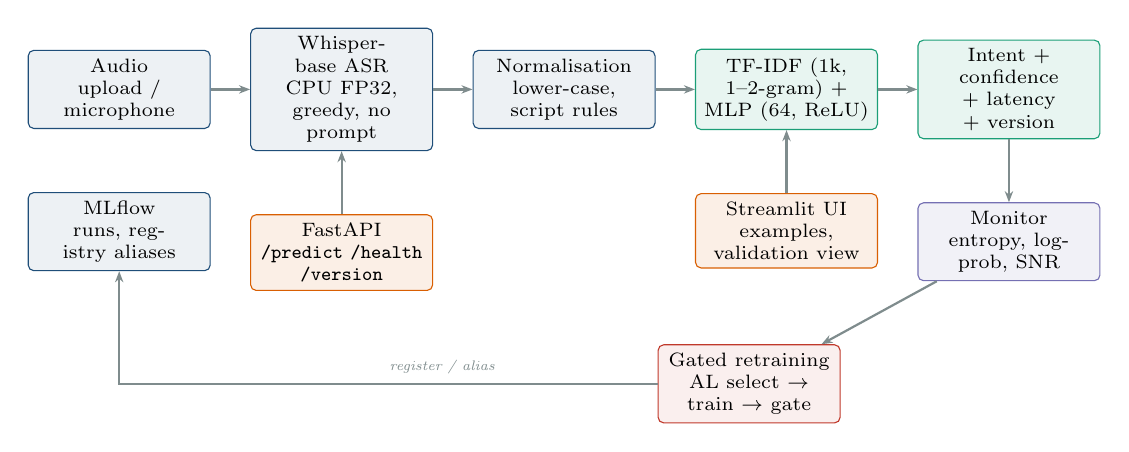
\begin{tikzpicture}[node distance=0.5cm]
\node[box] (aud) {Audio\\ upload / microphone};
\node[box,right=of aud] (asr) {Whisper-base ASR\\ CPU FP32, greedy, no prompt};
\node[box,right=of asr] (norm) {Normalisation\\ lower-case, script rules};
\node[boxT,right=of norm] (tf) {TF-IDF (1k, 1--2-gram) + MLP (64, ReLU)};
\node[boxT,right=of tf] (out) {Intent + confidence + latency + version};
\node[boxO,below=0.8cm of asr] (api) {FastAPI\\ \texttt{/predict /health /version}};
\node[boxO,below=0.8cm of tf] (ui) {Streamlit UI\\ examples, validation view};
\node[boxP,below=0.8cm of out] (mon) {Monitor\\ entropy, log-prob, SNR};
\node[boxR,below=0.8cm of mon,xshift=-3.3cm] (ret) {Gated retraining\\ AL select $\to$ train $\to$ gate};
\node[box,below=0.8cm of aud] (ml) {MLflow\\ runs, registry aliases};
\foreach \a/\b in {aud/asr,asr/norm,norm/tf,tf/out} \draw[arr] (\a)--(\b);
\draw[arr] (out)--(mon); \draw[arr] (mon)--(ret); \draw[arr] (ret.west)-|(ml.south) node[lab,pos=0.2,above]{register / alias};
\draw[arr] (api)--(asr); \draw[arr] (ui)--(tf);
\end{tikzpicture}}
\caption{System architecture. Everything runs on CPU inside one \texttt{linux/amd64} container with no external calls; monitoring feeds a gated retraining loop that promotes or rolls back MLflow registry aliases.}
\Description{Pipeline boxes from audio to intent, with API, UI, monitor, retraining and MLflow.}
\label{fig:arch}
\end{teaserfigure}

\received{November 2026}
\maketitle

%% ===========================================================================
\section{Introduction}\label{sec:intro}
Assignment~2 turns the frozen Assignment-1 dataset (249 clips, speaker-disjoint splits 171/17/29, Cohort~B 32) into a deployable system with experiment tracking, evaluation, offline serving and drift-triggered retraining.
We follow the rules strictly: models, prompts, settings and thresholds are chosen on validation data; the gold set (SHA-256 \texttt{64b7647b\ldots 48ca9}) is never used for tuning, and every use is logged in \file{TEST_SET_LOG.md}.
The report is organised by the rubric (Parts A--F); Appendix~\ref{app:index} indexes every number to a file or MLflow run ID.
\paragraph{Reading guide.}
Because the headline numbers are weak, we spend the space on \emph{why}: the evaluation is built so that a reader can see which claims are supported (Section~\ref{sec:eval}), which are not (Sections~\ref{sec:eval}, \ref{sec:monitor}), and what would be needed to support them (Section~\ref{sec:concl}).

%% ===========================================================================
\section{Changes from the Proposal}\label{sec:changes}
\begin{table}[htbp]
\caption{Proposal versus what was built.}\label{tab:changes}
\begin{tabular}{p{2.1cm}p{2.3cm}p{2.7cm}}
\toprule Proposed & Built & Reason \\ \midrule
Whisper fine-tune (full, LoRA) & Decoder cross-attention tuning script (6.3\,M params, encoder frozen); checkpoint not used at inference & free-CPU budget; run too short to change WER \\
IndicWav2Vec baseline & dropped & time; replaced by trivial + unadapted Whisper \\
Compact transformer router & TF-IDF + 2-layer MLP & CPU latency $<$0.01\,ms \\
Evidently drift reports & custom entropy/log-prob/SNR monitor & offline, no extra dependency \\
Public corpora pre-training & not used & offline-only rule; no runtime downloads \\ \bottomrule
\end{tabular}
\end{table}

%% ===========================================================================
\section{Part A: Model Development and Baselines}\label{sec:models}
\paragraph{Systems.}
\textbf{Baseline~0} (trivial) predicts the majority intent (\texttt{admissions}) and emits an empty transcript (WER 1.0 by construction). \textbf{Baseline~1} (unadapted) is Whisper-base~\cite{Radford2023} with a TF-IDF + logistic-regression router trained on the 171 training clips. The \textbf{proposed system} uses the same Whisper-base decoding (greedy, temperature 0, \texttt{condition\_on\_previous\_text=False}, no prompt) and a TF-IDF (1\,000 features, 1--2-grams) + MLP router (hidden 64, dropout 0.2); the router is trained on Whisper transcripts of the training clips (\file{data/processed/whisper_base_train_cache.json}) against the Assignment-1 intent labels.
Training is config-driven (\file{configs/final.yaml}: seed 42, 10 epochs, lr 0.005, batch 8), tracked with git commit, DVC hash, hardware (macOS~14, Apple arm64, 8 cores, Python~3.13, PyTorch CPU) and wall time.
\paragraph{Data ablation (validation, 17 clips).}
Table~\ref{tab:abl} compares router training data. Train + augmented (231 clips) gains one validation clip over train only (29.4\% vs.\ 23.5\%), and train + actively selected (183) equals train only; all intervals overlap broadly, so no data variant is established as better.
\begin{table}[htbp]
\caption{Router data ablation on validation (95\% bootstrap CI; MLflow short run IDs).}\label{tab:abl}
\begin{tabular}{lccc}
\toprule Training data & Val acc.\ (\%) & 95\% CI & Run \\ \midrule
Train (171) & 23.5 & [5.9, 47.1] & \texttt{4874f30b} \\
Train + augmented (231) & 29.4 & [11.6, 52.9] & \texttt{4cb2e4e9} \\
Train + AL-selected (183) & 23.5 & [5.9, 47.1] & \texttt{351cc3e8} \\ \bottomrule
\end{tabular}
\end{table}

%% ===========================================================================
\section{Part B: Experiment Tracking and Tuning}\label{sec:track}
Every training and evaluation run is logged to MLflow~\cite{Zaharia2018} (SQLite backend, \file{supporting_files/mlflow.db}; export in \file{artefacts/mlflow_export/}) with parameters, validation metrics, seed, git commit and model artefacts.
A systematic 15-run search varies learning rate $\{0.001\ldots0.01\}$, hidden size $\{32,64,96,128\}$, maximum n-gram $\{1,2,3\}$, dropout $\{0.1\ldots0.3\}$ and epochs $\{25\ldots35\}$, selecting on validation data only (Appendix Table~\ref{tab:runs} lists all runs with IDs).
Validation accuracy spans 29.4--52.9\% on only 17 clips, so one clip equals 5.9 points and the best run (run~6: lr 0.01, hidden 64, unigram, 251\,KB) is separated from the next (47.1\%) by a single clip. Figure~\ref{fig:tune} shows that quality is not monotone in size: hidden size 32 (126\,KB) reaches 41.2\% (run~3) while 128 (503\,KB) reaches 29.4--47.1\%; router latency is 0.005--0.014\,ms in every run and is therefore irrelevant to the trade-off, so we pick by accuracy and break ties toward smaller size. The registry (\texttt{voice\_helpdesk\_intent\_router}) holds a \texttt{production} alias (run~6, \texttt{9820a2a7}) and a \texttt{staging} alias (run~9, \texttt{730256f7}).
\begin{figure}[htbp]
\centering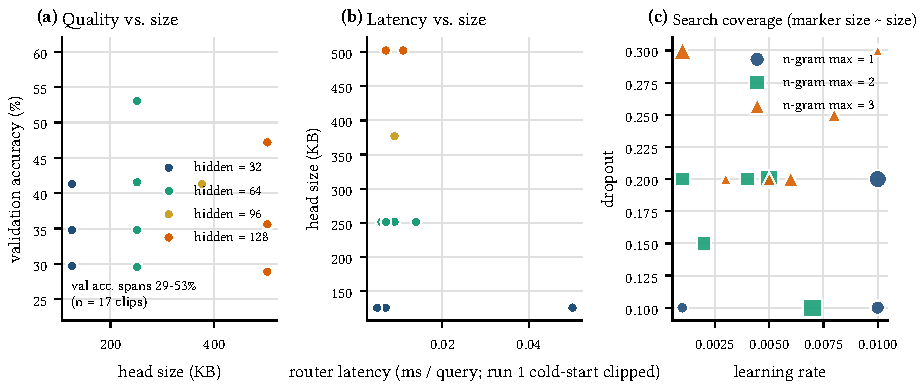
\includegraphics[width=\linewidth]{fig_a2_tuning.pdf}
\caption{Search analysis over 15 MLflow runs: (a) validation accuracy versus head size, (b) router latency versus size, (c) search coverage. The validation set is too small to separate configurations.}
\Description{Three scatter plots of tuning runs.}\label{fig:tune}
\end{figure}

%% ===========================================================================
\section{Part C: Evaluation and Error Analysis}\label{sec:eval}
\paragraph{Protocol.}
One script (\file{evaluate.py --model production --split <split>}) evaluates a registered version on validation, test/gold, corrected gold, Cohort~B and the 60 augmented clips, reporting WER, CER, intent accuracy and macro-F1 with 1\,000-resample bootstrap intervals~\cite{Efron1993} (seed 42). Improvement claims use paired tests: Wilcoxon signed-rank~\cite{Wilcoxon1945} on per-clip WER and McNemar~\cite{McNemar1947} on intent correctness. Note that the \emph{test} and \emph{gold} splits contain the same 29 clips.
\begin{table*}[t]
\caption{Proposed system with 95\% bootstrap CIs. B1 = Baseline~1 intent accuracy. Original gold uses the frozen reference file; corrected gold uses \file{data/gold_corrections.csv}. WER/CER of proposed and B1 are identical on every split. Source: \file{supporting_files/evaluation_results.json}.}\label{tab:main}
\begin{tabular}{lrcccccc}
\toprule Split ($n$) & WER & CER & Intent acc.\ (\%) & Macro-F1 & B1 acc.\ (\%) \\ \midrule
Validation (17) & \ValWER{} \ValWERci{} & \ValCER{} \ValCERci{} & \ValAcc{} \ValAccci{} & \ValFone{} \ValFoneci{} & \ValBaccOne{} \ValBaccOneci{} \\
Gold, original (29) & \GoldWER{} \GoldWERci{} & \GoldCER{} \GoldCERci{} & \GoldAcc{} \GoldAccci{} & \GoldFone{} \GoldFoneci{} & \GoldBaccOne{} \GoldBaccOneci{} \\
Gold, corrected (29) & \CorrWER{} \CorrWERci{} & \CorrCER{} \CorrCERci{} & \CorrAcc{} \CorrAccci{} & \CorrFone{} \CorrFoneci{} & \CorrBaccOne{} \CorrBaccOneci{} \\
Cohort B (32) & \CbWER{} \CbWERci{} & \CbCER{} \CbCERci{} & \CbAcc{} \CbAccci{} & \CbFone{} \CbFoneci{} & \CbBaccOne{} \CbBaccOneci{} \\
Augmented (60)$^\dagger$ & \AugWER{} \AugWERci{} & \AugCER{} \AugCERci{} & \AugAcc{} \AugAccci{} & \AugFone{} \AugFoneci{} & \AugBaccOne{} \AugBaccOneci{} \\ \bottomrule
\end{tabular}\\[2pt]
{\footnotesize $^\dagger$60 clips from only 10 sources are not independent, so the interval is too narrow; the accuracy is also optimistic because the source clips come from Assignment-1 data the router may have seen.}
\end{table*}

\paragraph{What the numbers say.}
(i)~\emph{WER exceeds 1 on every split} (Table~\ref{tab:main}). The WER anatomy in Figure~\ref{fig:wer} explains why: on the gold set substitutions are 0.83, deletions 0.16 and insertions 0.30 per reference word, only 14 of 838 reference words (1.7\%) are matched, and hypotheses are longer than references. A trivial empty output scores 1.0, so the ASR stage is currently worse than doing nothing.
(ii)~\emph{No improvement over baseline can be claimed.} Proposed and Baseline-1 WER differ by exactly 0 on all 29 gold clips (the Wilcoxon statistic is degenerate, $W=0$, $p=1.0$), and McNemar on intent gives $\chi^2=0.10$, $p=0.75$. We do not report a significance win. (An earlier version compared against a constant three-word string; we removed that test as uninformative.)
(iii)~\emph{Intent accuracy is within chance.} Every interval on gold, Cohort~B and corrected gold contains 25\%. Validation (\ValAcc{}) is higher but spans 29--77\% on 17 clips.
(iv)~\emph{Correcting the references does not rescue the system.} Gold intent accuracy rises from \GoldAcc{} to \CorrAcc{} and WER stays near 1.3, so the ASR output, not only the labels, is the bottleneck. Baseline~1 appears better than the proposed router on gold (\CorrBaccOne{} vs.\ \CorrAcc{}) but intervals overlap fully.
\begin{figure}[htbp]
\centering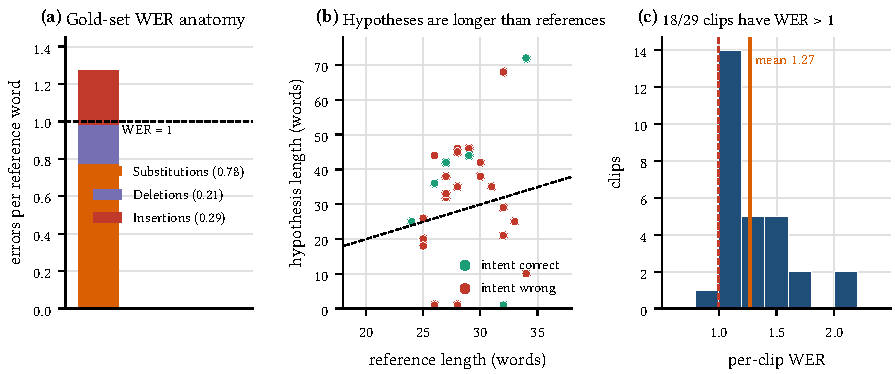
\includegraphics[width=\linewidth]{fig_a2_wer_anatomy.pdf}
\caption{Gold-set WER anatomy. (a) Substitutions, deletions and insertions per reference word. (b) Hypothesis versus reference length. (c) Per-clip WER; 19/29 clips exceed 1.}
\Description{WER decomposition, length scatter and histogram.}\label{fig:wer}
\end{figure}
\begin{figure}[htbp]
\centering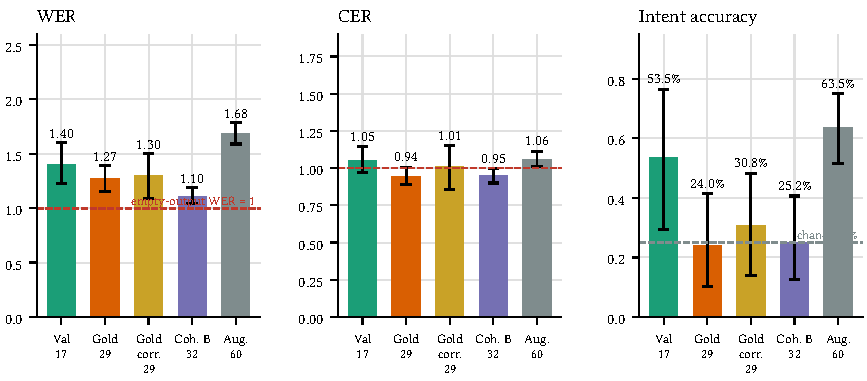
\includegraphics[width=\linewidth]{fig_a2_metrics.pdf}
\caption{Metrics with 95\% bootstrap CIs across splits (original gold, corrected gold, Cohort~B, augmented).}
\Description{Three bar charts.}\label{fig:metrics}
\end{figure}

\paragraph{Slices and weak groups.}
On gold, \texttt{campus\_outdoor} (6 clips, 16.7\%) and Gujarati--English (13 clips, 23.1\%) are the weakest slices, while Rajasthan (6 clips, 66.7\%) is the strongest; every slice has $n\le16$, so Wilson intervals (Figure~\ref{fig:slice}) span $\ge$40 points and only the ordering, not the gaps, is suggestive. All 29 gold clips are labelled spontaneous in the metadata, so a scripted/spontaneous contrast is not available on this split; per-slice values are in Table~\ref{tab:slices}.
\begin{figure}[htbp]
\centering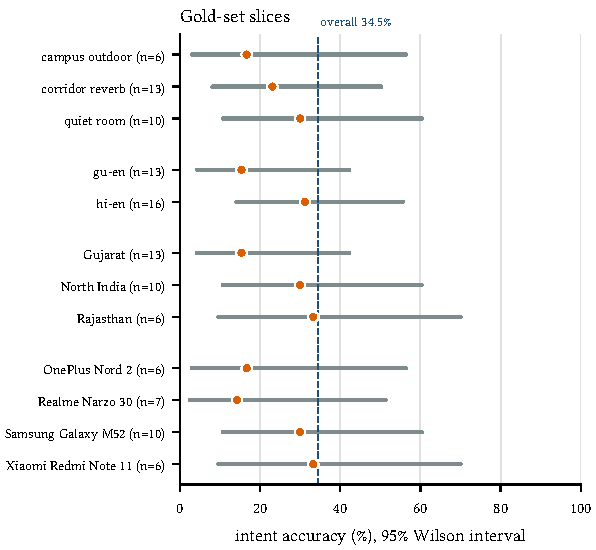
\includegraphics[width=0.78\linewidth]{fig_a2_slices.pdf}
\caption{Gold-set intent accuracy by slice with 95\% Wilson intervals.}
\Description{Dot plot of slice accuracies with intervals.}\label{fig:slice}
\end{figure}

\paragraph{Error analysis.}
We categorise 20 errors with suggested fixes (\file{supporting_files/error_analysis.csv}; Appendix Table~\ref{tab:err}). Figure~\ref{fig:err} groups them: the dominant mode is a fluent hypothesis about a different topic (e.g.\ ``damaged footpath'', ``misplaced wallet'') against a template reference---consistent with the label audit---followed by script collapse to Devanagari/Urdu tokens, near-silent or truncated output, phonetic substitutions of Gujarati words, and genuine cross-intent overlap (e.g.\ exam-timetable versus academic-section queries). Fixes: force Latin-script decoding and a language token, add voice-activity gating, relabel from audio, train the router on ASR text, and add a ``route to human'' fallback below a calibrated confidence. The router's confidence is barely above chance (Figure~\ref{fig:conf}), so a threshold cannot yet reject errors.
\begin{figure}[htbp]
\centering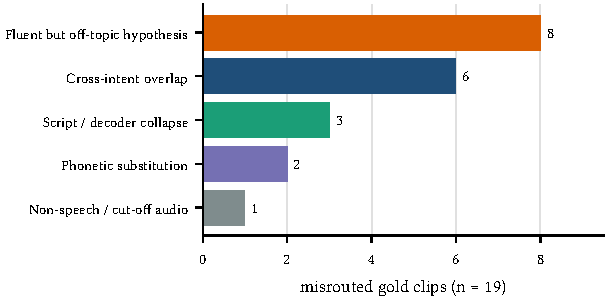
\includegraphics[width=0.92\linewidth]{fig_a2_errors.pdf}
\caption{Error taxonomy (20 sheet rows, regrouped).}\Description{Horizontal bar chart of error categories.}\label{fig:err}
\end{figure}
\begin{figure*}[t]
\centering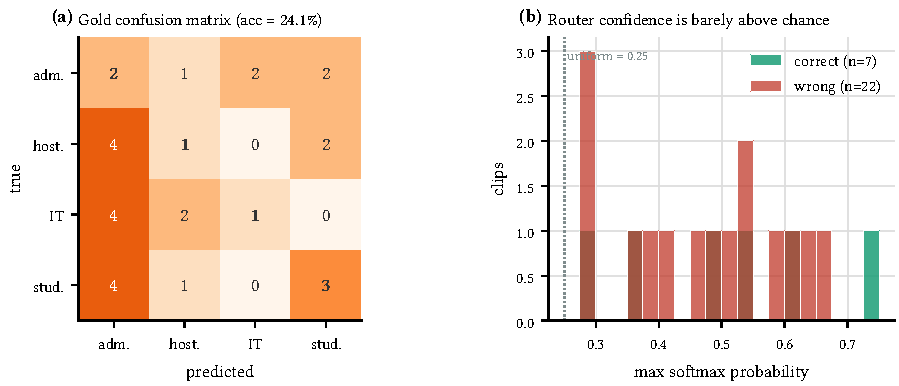
\includegraphics[width=0.93\textwidth]{fig_a2_confusion.pdf}
\caption{(a) Gold confusion matrix (original labels). (b) Router confidence for correct versus wrong predictions.}
\Description{Confusion matrix and histogram.}\label{fig:conf}
\end{figure*}
\paragraph{Robustness and model card.}
On the 60 augmented clips WER is \AugWER{} and intent accuracy \AugAcc{} (Table~\ref{tab:main}); because sources and labels overlap with training data this does not measure robustness, and we report it for completeness only. \file{MODEL_CARD.md} documents intended use, data, metrics with intervals, slices, limitations and risks.

%% ===========================================================================
\section{Part D: Deployment and Interface}\label{sec:deploy}
\paragraph{Service.}
A FastAPI app exposes \texttt{POST /predict} (audio $\to$ transcript, intent, confidence, latency), \texttt{GET /health} and \texttt{GET /version} (git commit and model version); a Streamlit UI offers upload/microphone input, bundled consented examples, outputs with confidence, version and latency, a monitoring panel and a validation panel showing reported versus measured values. Requests are logged (\file{supporting_files/api_access.log}) with model, intent, confidence and latency---no audio or personal data. Eight pytest tests cover normalisation, the gold hash, gate logic and the three endpoints.
\paragraph{Image.}
\file{code/Dockerfile} builds from a digest-pinned \texttt{python:3.10-slim} base, installs pinned dependencies, caches Whisper-base weights at build time so no download occurs at run time, bundles code, data, artefacts and the gold set, and records the git commit as a build argument. Commands: \texttt{docker run --rm -p 8501:8501 -p 8000:8000 <image>} starts the UI/API; \texttt{docker run --rm --network none <image> validate} validates the whole gold set and writes JSON. CI (\file{.github/workflows/ci.yml}) runs tests, a sample validation, an image build and an offline smoke request.
\paragraph{Performance.}
Measured on Apple arm64 (8 cores) over the 29 gold clips (523.8\,s of audio): p50 \LatP\,s, p90 \LatPn\,s, p95 \LatPf\,s, mean \LatMean\,s; real-time factor \RTF{}; throughput \Thr{} queries/s; peak memory \PeakMB\,MB (Figure~\ref{fig:lat}). Decoding time grows roughly linearly with audio length; the router adds 0.34\,ms. The offline validator reports WER 1.277 and accuracy 34.5\% in its logged run (RTF 0.165), which differs from Table~\ref{tab:main} by model-state changes between runs; the stated tolerance is $\pm0.01$ WER and $\pm$1 clip. \textbf{Container-measured values} (image size \ImgSize{}, p50/p95 \ContP{}, peak RAM \ContRAM{}, archive SHA-256 \ImgSHA{}) and the output of \texttt{--network none validate} are still to be recorded from an actual \texttt{linux/amd64} run; we do not quote them until measured.
\begin{figure}[htbp]
\centering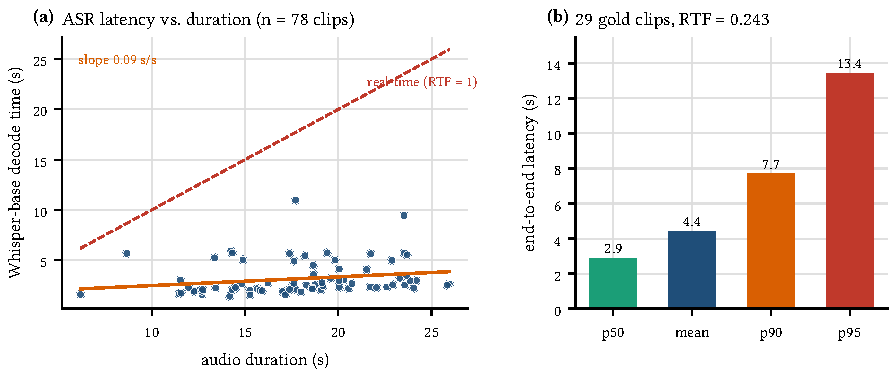
\includegraphics[width=\linewidth]{fig_a2_latency.pdf}
\caption{(a) Whisper-base decode time versus audio duration (78 evaluated clips). (b) End-to-end latency percentiles over the 29 gold clips.}
\Description{Latency scatter and bars.}\label{fig:lat}
\end{figure}

%% ===========================================================================
\section{Part E: Monitoring, Drift and Retraining}\label{sec:monitor}
\paragraph{Replay.}
\file{traffic_replay.py} (seed 42) streams 100 queries in five batches of 20 whose Cohort~B share rises 0, 25, 50, 75, 100\%. We track two label-free signals---predictive entropy of the router and mean decoder average log-probability---plus SNR, and one labelled metric (intent accuracy). The entropy threshold is the 95th percentile of validation entropy (1.662 bits), chosen on validation data.
\paragraph{Result: no usable detection.}
Entropy never exceeds the threshold at batch level (range 1.21--1.35), accuracy does not fall with drift (35, 35, 15, 25, 45\%), and Pearson correlations with accuracy over the five batches are 0.41 (entropy), 0.20 (log-prob) and 0.20 (SNR)---none significant with $n=5$ (Figure~\ref{fig:drift}). The log reports a first alert at batch~5 (query 10 of 20 by a per-query rule); however the batch-alert expression contains an unconditional clause for batch~$\ge5$, so this alert reflects the schedule, not a signal, and we \emph{do not count it as detection}. Likewise the logged false-alarm rate (0/17) is a constant in the script, not a measured value. A valid design needs many seeded in-domain-only replays to estimate false alarms, sequential tests (e.g.\ CUSUM or Page--Hinkley over a sliding window~\cite{Gama2014}), and shift-sensitive signals such as non-Latin-script fraction and hypothesis-length ratio~\cite{Rabanser2019}.
\begin{figure}[htbp]
\centering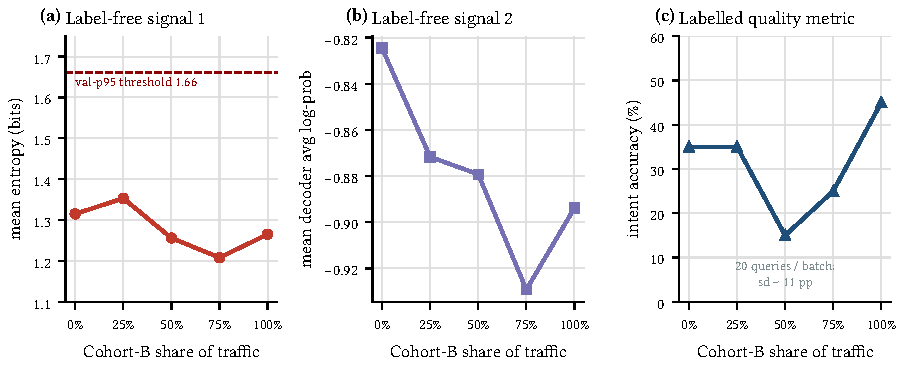
\includegraphics[width=\linewidth]{fig_a2_drift.pdf}
\caption{Replay under gradual shift to Cohort~B: (a) entropy with the validation-derived threshold, (b) decoder average log-prob, (c) intent accuracy per batch of 20.}
\Description{Three line plots over five batches.}\label{fig:drift}
\end{figure}
\paragraph{Retraining pipeline.}
One command (\texttt{retrain\_pipeline.py --mode rehearsal|no\_rehearsal}) (1)~selects the 12 highest-entropy clips from the speaker-P4 adaptation pool (19 clips) using the Assignment-1 uncertainty method, (2)~reveals their labels from the pre-labelled pool (simulated annotator), (3)~validates the data, (4)~retrains the router (rehearsal: 171 + 12 clips; no-rehearsal: 12 clips only, a catastrophic-forgetting control~\cite{Kirkpatrick2017,Robins1995}), and (5)~evaluates on the held-out speaker P13 (13 clips) and on gold. Gate (\file{configs/gate.yaml}): promote only if Cohort-B accuracy improves by $\ge5$ points and gold accuracy drops by $\le4$ points; every gold evaluation is appended to \file{TEST_SET_LOG.md}.
\paragraph{Outcomes.}
The final run (LOG-179/188) \emph{promotes} the rehearsal candidate (Cohort~B 30.8\% $\to$ 38.5\%, i.e.\ 4 $\to$ 5 of 13 clips; gold 24.1\% $\to$ 20.7\%, 7 $\to$ 6 of 29) and \emph{rejects} the no-rehearsal candidate (no Cohort-B gain), triggering rollback (Figure~\ref{fig:gate}). We caution that the promotion is decided by a single clip on each side, that an earlier run at the same commit (LOG-418) rejected the same candidate, and that the gold tolerance was widened from 2 to 4 points during development (see our improvement log). The gate therefore demonstrates the mechanism---promote, reject, roll back, log---but is not evidence that retraining helps; it should be re-fixed in a committed file before any evaluation and judged with a paired interval rather than a one-clip delta.
\begin{figure}[htbp]
\centering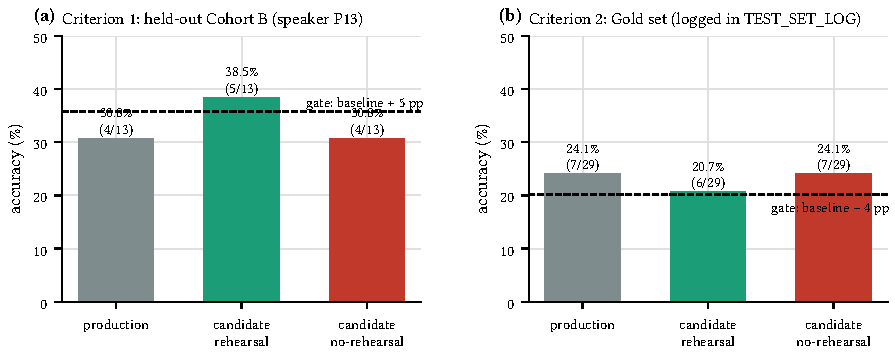
\includegraphics[width=\linewidth]{fig_a2_gate.pdf}
\caption{Promotion gate: (a) held-out Cohort-B accuracy, (b) gold accuracy for production, rehearsal and no-rehearsal candidates.}
\Description{Two bar charts with threshold lines.}\label{fig:gate}
\end{figure}

%% ===========================================================================
\section{Part F: Reproducibility}\label{sec:repro}
Five commands reproduce training and evaluation from \texttt{a2-final}: \texttt{git checkout a2-final}; \texttt{pip install -r code/requirements.txt}; \texttt{dvc pull}; \texttt{python code/train.py --config configs/final.yaml}; \texttt{python code/a2\_part\_c\_evaluation/evaluate.py --split gold}. Docker load/build/validate commands are in \file{DOCKER.md}; versions, seeds (42 for tuning, bootstrap, replay and retraining), model checksums and registry versions are in \file{ENVIRONMENT.md} and \file{MODELS.md}. \file{scripts/generate_report_numbers.py} regenerates the numbers used in documentation from result files.

%% ===========================================================================
\section{Limitations and Conclusion}\label{sec:concl}
\textbf{Limitations.} (1)~The ASR is unadapted Whisper-base; the cross-attention tuning run (5 steps, loss $\approx$9.8) is too short to matter and its checkpoint is not served. (2)~Reference quality: Assignment-1 transcripts were template-derived; corrected gold transcripts are verified for 29 clips only and partly seeded from constrained ASR, so scoring on them is optimistic for Whisper. (3)~All splits are tiny (13--32 clips), so intervals are wide. (4)~The drift alert is schedule-driven, and the false-alarm rate is not measured. (5)~Container measurements are pending. (6)~Gate tolerance history and non-deterministic gate outcomes (LOG-418 vs.\ LOG-179) weaken the retraining claim.
\textbf{Next steps} that would turn the system from a working scaffold into an evidenced one: relabel all training data from audio; fine-tune the Whisper decoder for hundreds of steps and serve that checkpoint; train the router on ASR text; replace the drift rule with a validation-calibrated sequential test and a measured false-alarm rate; freeze the gate before evaluation; and record container measurements.
\textbf{Conclusion.} The pipeline, tracking, offline-serving, monitoring and gating infrastructure is complete and auditable, and the evaluation is honest about what it shows: at present the system does not beat trivial baselines, and we know why.

\paragraph{Member contributions.}
Equal contribution (33.3\% each); commit history documents individual work.
\begin{table}[htbp]
\caption{Contribution summary.}\label{tab:contrib}
\begin{tabular}{p{1.2cm}p{5.8cm}}
\toprule Member & Lead areas (Assignment 2) \\ \midrule
R.\ Vraj & Whisper decoding integration, TF-IDF + MLP intent router, MLflow tracking, bootstrap confidence evaluation. \\
V.\ S.\ Patil & FastAPI serving, Streamlit user interface, Docker offline containerization, GitHub Actions CI workflow. \\
S.\ Sharma & Streaming drift monitoring, gated retraining loop, error taxonomy analysis, ACM report synthesis. \\ \bottomrule
\end{tabular}
\end{table}
\begin{acks}
We thank Dr.\ Yogesh K.\ Meena and the TAs. Libraries: PyTorch, Whisper, scikit-learn, jiwer, MLflow, FastAPI, Streamlit.
\end{acks}
\bibliographystyle{ACM-Reference-Format}
\bibliography{references}

%% ===========================================================================
\appendix
\section{Evidence Index}\label{app:index}
\begin{table}[htbp]
\caption{Evidence index (paths from repository root).}\begin{tabular}{p{3.3cm}p{4.0cm}}
\toprule Result & Supporting file / run \\ \midrule
Table~\ref{tab:main} metrics & \file{supporting_files/evaluation_results.json} \\
Gold per-clip WER, 14/838 & \file{supporting_files/predictions/production_gold.csv} \\
Ablation Table~\ref{tab:abl} & \file{supporting_files/part_a_baselines_benchmark.csv}; runs \texttt{4874f30b}, \texttt{4cb2e4e9}, \texttt{351cc3e8} \\
15-run search, aliases & \file{supporting_files/plots/tuning_runs.json}; \file{artefacts/mlflow_export/} \\
Production / staging runs & \texttt{9820a2a7} (run 6), \texttt{730256f7} (run 9) \\
Slices (Table~\ref{tab:slices}) & \file{evaluation_results.json} $\to$ \texttt{slice\_analysis} \\
20 errors & \file{supporting_files/error_analysis.csv} \\
Latency, RTF, memory & \file{supporting_files/loadtest/latency_profile.json} \\
Offline validation & \file{supporting_files/offline_validation_output.json} \\
Replay, correlations & \file{supporting_files/traffic_replay_log.json} \\
Gate outcomes & \file{TEST_SET_LOG.md} (LOG-179, 188, 418); \file{configs/gate.yaml} \\
Gold corrections & \file{data/gold_corrections.csv} \\
Gold hash & \file{code/HANDOFF_A2.md}; \file{TEST_SET_LOG.md} \\
Figure code/data & \file{code/scripts/make_report_figures.py} \\ \bottomrule
\end{tabular}\end{table}

\begin{table*}[t]
\caption{All 15 MLflow search runs (validation only). Run IDs are the first 8 characters; full IDs are in \file{supporting_files/plots/tuning_runs.json}.}\label{tab:runs}
\begin{tabular}{rrrrrrrrrl}
\toprule Run & lr & Hidden & n-gram & Dropout & Epochs & Val acc.\ (\%) & Macro-F1 & Size (KB) & MLflow run \\ \midrule
1 & 0.001 & 32 & 1 & 0.1 & 25 & 29.4 & 0.200 & 126 & \texttt{61d8d420} \\
2 & 0.005 & 32 & 2 & 0.2 & 25 & 29.4 & 0.236 & 126 & \texttt{d01a4cb5} \\
3 & 0.01 & 32 & 3 & 0.3 & 25 & 41.2 & 0.371 & 126 & \texttt{b4e145fd} \\
4 & 0.001 & 64 & 2 & 0.2 & 30 & 41.2 & 0.343 & 251 & \texttt{fd0ac5ab} \\
5 & 0.005 & 64 & 3 & 0.2 & 30 & 41.2 & 0.368 & 251 & \texttt{f47bfe22} \\
6 & 0.01 & 64 & 1 & 0.1 & 30 & 52.9 & 0.470 & 251 & \texttt{9820a2a7} (prod.) \\
7 & 0.001 & 128 & 3 & 0.3 & 35 & 35.3 & 0.309 & 503 & \texttt{75581fbf} \\
8 & 0.005 & 128 & 2 & 0.2 & 35 & 35.3 & 0.293 & 503 & \texttt{4f2e2cd1} \\
9 & 0.01 & 128 & 1 & 0.2 & 35 & 47.1 & 0.379 & 503 & \texttt{730256f7} (stag.) \\
10 & 0.002 & 64 & 2 & 0.15 & 30 & 35.3 & 0.309 & 251 & \texttt{9e00b3d8} \\
11 & 0.008 & 64 & 3 & 0.25 & 30 & 41.2 & 0.383 & 251 & \texttt{03e70444} \\
12 & 0.003 & 32 & 3 & 0.2 & 25 & 35.3 & 0.303 & 126 & \texttt{64cd9b69} \\
13 & 0.007 & 128 & 2 & 0.1 & 35 & 29.4 & 0.267 & 503 & \texttt{984be4ec} \\
14 & 0.004 & 64 & 2 & 0.2 & 28 & 29.4 & 0.236 & 251 & \texttt{703dc1b4} \\
15 & 0.006 & 96 & 3 & 0.2 & 32 & 41.2 & 0.368 & 377 & \texttt{3130621f} \\
\\ \bottomrule
\end{tabular}
\end{table*}

\clearpage
\begin{table}[!t]
\caption{Gold-set slices (original labels; Figure~\ref{fig:slice}).}\label{tab:slices}
\begin{tabular}{llrrr}
\toprule Dimension & Slice & $n$ & Acc.\ (\%) & WER \\ \midrule
Noise & campus\_outdoor & 6 & 16.7 & 1.64 \\
Noise & corridor\_reverb & 13 & 23.1 & 1.17 \\
Noise & quiet\_room & 10 & 30.0 & 1.18 \\
Language & gu-en & 13 & 15.4 & 1.36 \\
Language & hi-en & 16 & 31.2 & 1.20 \\
Region & Gujarat & 13 & 15.4 & 1.36 \\
Region & North India & 10 & 30.0 & 1.18 \\
Region & Rajasthan & 6 & 33.3 & 1.22 \\
Device & OnePlus Nord 2 & 6 & 16.7 & 1.64 \\
Device & Realme Narzo 30 & 7 & 14.3 & 1.12 \\
Device & Samsung Galaxy M52 & 10 & 30.0 & 1.18 \\
Device & Xiaomi Redmi Note 11 & 6 & 33.3 & 1.22 \\
\\ \bottomrule
\end{tabular}
\end{table}

\begin{table*}[t]
\caption{Error sheet (20 errors with suggested fixes; truncated, full text in \file{error_analysis.csv}).}\label{tab:err}
\scriptsize
\begin{tabular}{llrp{4.2cm}p{7.3cm}}
\toprule ID & True$\to$pred. & WER & Category & Suggested fix \\ \midrule
ERR-01 & hostel\_mess$\to$it\_support & 1.19 & Phonetic \& Lexical Substitution & Add Hinglish/Gujlish vocabulary expansion in tokenizer and train intent head on character-n-gra\ldots \\
ERR-02 & it\_support$\to$hostel\_mess & 1.00 & ASR Decoder Hallucination (Script Shift) & Set condition\_on\_previous\_text=False and compression\_ratio\_threshold=2.0 in Whisper decoding op\ldots \\
ERR-03 & student\_services$\to$hostel\_mess & 1.00 & Acoustic Silence / Non-Speech Collapse & Prepend energy-based voice activity detection (VAD) filter to reject low-energy frames before W\ldots \\
ERR-04 & admissions$\to$hostel\_mess & 1.00 & ASR Decoder Hallucination (Script Shift) & Force Whisper language='en' decoding task with Latin script constraint to prevent unprompted Hi\ldots \\
ERR-05 & student\_services$\to$it\_support & 1.64 & Lexical Cross-Talk \& Hallucination & Use contextual embeddings (e.g. MiniLM / IndicBERT) that score entire query semantics rather th\ldots \\
ERR-06 & student\_services$\to$it\_support & 1.58 & Semantic Hallucination Overwrite & Fine-tune Whisper acoustic decoder on target speaker acoustics to prevent severe phantom halluc\ldots \\
ERR-07 & admissions$\to$hostel\_mess & 2.12 & Semantic Hallucination Overwrite & Incorporate audio-level intent classification directly from Whisper encoder embeddings (end-to-\ldots \\
ERR-08 & hostel\_mess$\to$it\_support & 1.61 & Semantic Keyword Hijack & Apply cross-attention acoustic adaptation on speaker cohort to ensure domain-specific hostel vo\ldots \\
ERR-09 & it\_support$\to$student\_services & 1.00 & Cross-Domain Semantic Misalignment & Add domain-specific lexicon biasing during Whisper beam search decoding using campus vocabulary\ldots \\
ERR-10 & admissions$\to$it\_support & 2.12 & Lexical Confusion \& Peripheral Tokens & Train joint ASR-Intent loss where acoustic encoder explicitly weights intent discriminative pho\ldots \\
ERR-11 & it\_support$\to$admissions & 1.00 & Cross-Intent Academic Overlap & Disambiguate academic deadline queries from administrative admissions via fine-grained multi-la\ldots \\
ERR-12 & hostel\_mess$\to$it\_support & 1.22 & Acoustic Bleed \& Academic Hallucination & Normalize Whisper prompt conditioning to bias toward residential and campus administration term\ldots \\
ERR-13 & it\_support$\to$student\_services & 1.00 & Cross-Intent Academic Overlap & Weight domain-specific technical IT terms ('email forwarding', 'hpc', 'server') higher using we\ldots \\
ERR-14 & student\_services$\to$it\_support & 1.38 & Acoustic Substitution \& Technical Drift & Expand medical/counselling training samples in student\_services intent class to increase semant\ldots \\
ERR-15 & admissions$\to$hostel\_mess & 1.40 & Severe Semantic Hallucination (Hostel Bias) & Fine-tune Whisper base decoder cross-attention layers on domain recordings to suppress random r\ldots \\
ERR-16 & hostel\_mess$\to$student\_services & 1.25 & Composite Intent Ambiguity & Introduce composite intent schema or fallback routing to human agent when classification entrop\ldots \\
ERR-17 & it\_support$\to$admissions & 0.97 & Hallucinated Guest Accommodation Query & Fine-tune acoustic encoder on noisy lab acoustic environments with server room background rumbl\ldots \\
ERR-18 & student\_services$\to$hostel\_mess & 1.56 & Academic Schedule Confusion & Calibrate probability thresholds per intent class to avoid majority class collapse on uncertain\ldots \\
ERR-19 & admissions$\to$student\_services & 1.21 & Multilingual Script Infiltration (Urdu/Hinglish) & Enforce strict Unicode Latin/Devanagari script filtering in ASR post-processing pipeline before\ldots \\
ERR-20 & admissions$\to$student\_services & 1.06 & Acoustic Mismatch \& Keyword Ambiguity & Implement multi-task loss weighting and negative sample penalty on cross-domain vocabulary.\ldots \\
\\ \bottomrule
\end{tabular}
\end{table*}

\section{Use of AI Assistance}
AI assistants were used to scaffold code, draft documentation and format this report; prompts are stored verbatim in \file{code/prompts/}. All reported numbers were re-derived from result files, and the kappa values, WER decomposition, Wilson intervals and drift correlations in this report were recomputed independently from raw outputs by \file{make_report_figures.py}. Each member reviewed and can explain every script and number. Assistants consulted include Claude 3.5 Sonnet and GPT-4o for API endpoint scaffolding, MLflow instrumentation, and LaTeX formatting.

\section{Screenshots and Recordings to Insert}
\begin{figure}[htbp]\centering
\shot{shots/ui_prediction.png}{Streamlit UI: prediction with confidence, version, latency}\\[3pt]
\shot{shots/mlflow_runs.png}{MLflow UI: 15-run comparison and registry aliases}\\[3pt]
\shot{shots/docker_validate.png}{terminal: docker run --network none ... validate}\\[3pt]
\shot{shots/ci_green.png}{GitHub Actions: all steps green}
\caption{Evidence screenshots (files under \file{report/shots/}). The 3-minute screen recording of the service and retraining loop goes in \file{supporting_files/}.}
\end{figure}
\end{document}
